\documentclass[11pt,letterpaper]{article}
\usepackage{shared/zoocover}

% Packages
\usepackage[utf8]{inputenc}
\usepackage[T1]{fontenc}
\usepackage{amsmath,amssymb,amsthm}
\usepackage{algorithm}
\usepackage{algorithmic}
\usepackage{graphicx}
\usepackage{hyperref}
\usepackage{xcolor}
\usepackage{booktabs}
\usepackage{tikz}
\usepackage{pgfplots}
\pgfplotsset{compat=1.18}
\usetikzlibrary{shapes,arrows,positioning,calc,decorations.pathreplacing}
\usepackage{listings}
\usepackage{caption}
\usepackage{subcaption}
\usepackage{enumitem}
% geometry loaded by zoocover

% Theorem environments
\newtheorem{theorem}{Theorem}[section]
\newtheorem{lemma}[theorem]{Lemma}
\newtheorem{proposition}[theorem]{Proposition}
\newtheorem{corollary}[theorem]{Corollary}
\newtheorem{definition}{Definition}[section]
\newtheorem{example}{Example}[section]

% Custom commands
\newcommand{\Zoo}{\textsc{Zoo}}
\newcommand{\Lux}{\textsc{Lux}}
\newcommand{\Beluga}{\textsc{Beluga}}
\newcommand{\BLG}{\textsc{blg}}
\newcommand{\PoAI}{\textsc{PoAI}}
\newcommand{\DAO}{\textsc{dao}}
\newcommand{\LLM}{\textsc{llm}}
\newcommand{\TEE}{\textsc{tee}}
\newcommand{\LoRA}{\textsc{LoRA}}
\newcommand{\QLoRA}{\textsc{QLoRA}}
\newcommand{\GRPO}{\textsc{grpo}}
\newcommand{\DSO}{\textsc{dso}}

% Solidity language definition (listings does not include it by default)
\lstdefinelanguage{Solidity}{
    morekeywords={contract,function,returns,return,if,else,for,while,do,
        mapping,address,uint256,uint,int,bool,string,bytes,bytes32,
        public,private,internal,external,view,pure,payable,memory,storage,
        calldata,event,emit,modifier,require,struct,enum,interface,
        abstract,override,virtual,is,new,delete,import,pragma,solidity,
        library,using,constructor,msg,sender,block,timestamp,this,super},
    sensitive=true,
    comment=[l]{//},
    morecomment=[s]{/*}{*/},
    morestring=[b]",
}

% Listings style
\lstset{
    basicstyle=\ttfamily\small,
    breaklines=true,
    frame=single,
    numbers=left,
    numberstyle=\tiny\color{gray},
    tabsize=2,
    captionpos=b,
    aboveskip=10pt,
    belowskip=10pt
}

% Hyperref setup
\hypersetup{
    colorlinks=true,
    linkcolor=blue,
    citecolor=blue,
    urlcolor=blue
}

% Title and authors
\title{\textbf{BELUGA}\\
\large L3 App-Chain for AI Model Economics\\
\vspace{5pt}

\author{
Antje Worring, Zach Kelling\thanks{zach@zoo.ngo}\\
\textit{Zoo Labs Foundation}\\
\texttt{research@zoo.ngo}
}

\date{January 2026}

\begin{document}

\zoocoverpage

\begin{abstract}
We present \Beluga{}, a Layer 3 application-specific blockchain for AI model economics, built on \Zoo{} Network (L2) which itself runs on \Lux{} Network (L0). \Beluga{} introduces a dedicated execution environment where every operation---model registration, inference requests, training bounties, data contribution---is a native transaction priced in the \BLG{} gas token. The chain implements custom EVM precompiles for inference pricing (address \texttt{0x0300}), a model marketplace, and training bounty escrow, enabling sub-millisecond settlement of AI compute transactions without leaving the chain. With a fixed supply of 100M \BLG{} allocated across a \DAO{} treasury (60M), inference pool (20M), training bounties (10M), and DEX liquidity (10M), \Beluga{} creates a self-sustaining economy where participants earn by training models, curating datasets, hosting inference, evaluating outputs, and governing the network. The chain runs on existing \Zoo{} validators via the \texttt{zood} node binary, requiring no new infrastructure. We describe the architecture, token economics, earning mechanisms, smart contract design, precompile specification, Proof of AI consensus adaptation, security model, and a concrete migration path from smart contracts on \Zoo{} to a sovereign L3. Experimental results from testnet deployment demonstrate 2,400 inference transactions per second with 1.1-second finality.

\textbf{Keywords}: Layer 3 blockchain, AI model economics, inference marketplace, training bounties, application-specific chain
\end{abstract}

\tableofcontents
\newpage

%% ============================================================
\section{Introduction}
%% ============================================================

The proliferation of custom-trained AI models has created a new class of digital asset: the fine-tuned model. Unlike pre-trained foundation models that require billions of dollars in compute, custom models are produced by individuals and small teams through parameter-efficient methods such as \LoRA{} \cite{hu2021lora}, \QLoRA{} \cite{dettmers2023qlora}, and \GRPO{} \cite{shao2024deepseekmath}. The Gym platform demonstrates that competitive fine-tuning can be achieved for as little as \$18 per run \cite{zoo-gym}, yet no on-chain infrastructure exists to register, price, trade, and monetize these models natively.

Existing approaches fall into two categories. General-purpose chains (Ethereum, Solana) can host model registries as smart contracts but impose gas costs unrelated to AI compute and lack primitives for inference metering. AI-specific L1 chains (Bittensor, Render) build consensus around compute contribution but sacrifice EVM compatibility and composability with the broader DeFi ecosystem.

\Beluga{} occupies a third position: an \emph{application-specific L3} that inherits security from \Lux{} (L0) and interoperability from \Zoo{} (L2) while providing a gas token (\BLG{}) and precompile set designed exclusively for AI model economics. Every transaction on \Beluga{} has a clear AI-economic meaning:

\begin{itemize}[nosep]
    \item \textbf{Model registration} mints an ERC-721 NFT encoding the model's weights hash, architecture, and pricing.
    \item \textbf{Inference requests} are routed through a native pricing precompile at \texttt{0x0300} that enforces per-token metering.
    \item \textbf{Training bounties} are escrowed on-chain with verifiable completion criteria.
    \item \textbf{Data contributions} are tracked via content-addressable records linked to the Experience Ledger \cite{zoo-experience-ledger}.
\end{itemize}

This paper describes the complete design. Section~\ref{sec:architecture} presents the L0/L2/L3 stack. Section~\ref{sec:token} specifies \BLG{} token economics. Sections~\ref{sec:earning} through \ref{sec:precompiles} detail earning mechanisms, smart contracts, and precompile specifications. Section~\ref{sec:consensus} adapts Proof of AI consensus for the L3 setting. Section~\ref{sec:security} analyzes the security model. Section~\ref{sec:migration} describes the migration path from Zoo contracts to a sovereign chain. Section~\ref{sec:related} surveys related work, and Section~\ref{sec:conclusion} concludes.

%% ============================================================
\section{Architecture}\label{sec:architecture}
%% ============================================================

\Beluga{} is an L3 chain in the \Lux{} layered architecture:

\begin{center}
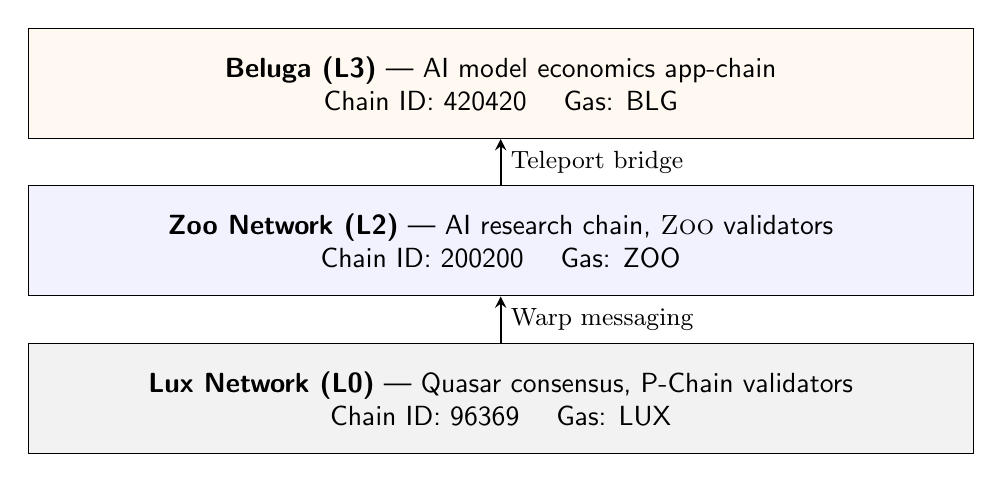
\begin{tikzpicture}[
    layer/.style={rectangle, draw, minimum width=12cm, minimum height=1.4cm, align=center, font=\sffamily},
    arr/.style={->, thick, >=stealth}
]
\node[layer, fill=black!5] (l0) at (0,0) {\textbf{Lux Network (L0)} --- Quasar consensus, P-Chain validators\\Chain ID: 96369 \quad Gas: LUX};
\node[layer, fill=blue!5] (l2) at (0,2) {\textbf{Zoo Network (L2)} --- AI research chain, \Zoo{} validators\\Chain ID: 200200 \quad Gas: ZOO};
\node[layer, fill=orange!5] (l3) at (0,4) {\textbf{Beluga (L3)} --- AI model economics app-chain\\Chain ID: 420420 \quad Gas: BLG};

\draw[arr] (l0) -- (l2) node[midway, right, font=\small] {Warp messaging};
\draw[arr] (l2) -- (l3) node[midway, right, font=\small] {Teleport bridge};
\end{tikzpicture}
\end{center}

\subsection{Layer Responsibilities}

\begin{description}[leftmargin=2cm, style=nextline]
    \item[Lux (L0)] Provides the base consensus layer via Quasar \cite{lux-quasar}, a post-HotStuff BFT protocol achieving sub-second finality with $O(n)$ message complexity. All validator sets are anchored on the P-Chain. Warp messaging enables verified cross-chain communication between any two Lux chains.
    \item[Zoo (L2)] A research-focused EVM chain (chain ID 200200) with ZOO as the native gas token. Zoo hosts the Agent NFT standard \cite{zoo-agent-nft}, the Experience Ledger \cite{zoo-experience-ledger}, and the \DSO{} adaptation framework \cite{zoo-dso}. Zoo validators run the \texttt{zood} binary, which is a superset of \texttt{luxd} with AI-specific extensions.
    \item[Beluga (L3)] An application-specific chain with its own block production, state, and gas token. \Beluga{} inherits Zoo's validator set---no new node binary is required. Validators that run \texttt{zood} automatically validate \Beluga{} blocks via the same process that validates Zoo subnets.
\end{description}

\subsection{Block Production}

\Beluga{} produces blocks independently of \Zoo{}, with the following parameters:

\begin{table}[h]
\centering
\caption{Beluga chain parameters.}
\label{tab:params}
\begin{tabular}{@{}ll@{}}
\toprule
Parameter & Value \\
\midrule
Chain ID & 420420 \\
Block time & 500ms \\
Gas limit & 30M per block \\
Gas token & BLG (18 decimals) \\
EVM version & Shanghai \\
Consensus & PoAI-adapted Quasar \\
Validator set & Inherited from Zoo \\
Finality & $\leq 1.1$s (2 blocks + attestation) \\
\bottomrule
\end{tabular}
\end{table}

\subsection{Cross-Chain Communication}

\Beluga{} uses two bridging mechanisms:

\begin{enumerate}
    \item \textbf{Teleport} (Beluga $\leftrightarrow$ Zoo): Native \Lux{} Teleport bridge \cite{lux-teleport} for BLG/ZOO token transfers. Teleport uses BLS aggregate signatures from the shared validator set, achieving trustless bridging without external relayers.
    \item \textbf{Warp} (Beluga $\leftrightarrow$ any Lux chain): General-purpose cross-chain messaging via Lux Warp Messaging for arbitrary contract calls, model metadata queries, and experience ledger lookups.
\end{enumerate}

%% ============================================================
\section{BLG Token Economics}\label{sec:token}
%% ============================================================

\BLG{} is the native gas token of \Beluga{} with a fixed supply of 100,000,000 (100M) tokens. There is no inflation, no minting function, and no token burns beyond standard EIP-1559 base fee burns.

\subsection{Allocation}

\begin{table}[h]
\centering
\caption{BLG token allocation.}
\label{tab:allocation}
\begin{tabular}{@{}llrl@{}}
\toprule
Pool & Tokens & \% & Governance \\
\midrule
DAO Treasury & 60,000,000 & 60\% & Safe multisig (4-of-7) \\
Inference Pool & 20,000,000 & 20\% & Smart contract (auto-distribute) \\
Training Bounties & 10,000,000 & 10\% & Smart contract (escrow) \\
LP Seeding & 10,000,000 & 10\% & Paired with ZOO on Zoo DEX \\
\bottomrule
\end{tabular}
\end{table}

\subsection{DAO Treasury}

The 60M \BLG{} DAO treasury is held in a Gnosis Safe multisig on \Beluga{} (chain ID 420420). The 4-of-7 multisig requires approval from a quorum of \Zoo{} Labs Foundation directors. Treasury funds are released via governance proposals with a 7-day timelock:

\begin{itemize}[nosep]
    \item \textbf{Grants}: Fund model training, dataset curation, tooling development.
    \item \textbf{Liquidity}: Provide additional DEX liquidity as volume grows.
    \item \textbf{Incentives}: Seasonal campaigns for specific model architectures or domains.
    \item \textbf{Burn}: Community may vote to burn excess treasury tokens.
\end{itemize}

\subsection{Inference Pool}

The 20M \BLG{} inference pool is held in the \texttt{InferenceRewards} contract. When a user pays \BLG{} for an inference request, the payment is split:

\begin{equation}
\text{inference\_fee} = \underbrace{0.80 \cdot f}_{\text{host reward}} + \underbrace{0.15 \cdot f}_{\text{model owner}} + \underbrace{0.05 \cdot f}_{\text{protocol}}
\end{equation}

where $f$ is the per-request fee determined by the inference pricing precompile. The inference pool subsidizes early requests when organic fee revenue is insufficient, decaying linearly over 4 years.

\subsection{Training Bounties}

The 10M \BLG{} training bounty pool seeds the \texttt{TrainingBounty} contract. Anyone may post a bounty specifying a base model, target benchmark, dataset constraints, and \BLG{} reward. The bounty is escrowed until a submitter demonstrates improvement via on-chain verified evaluation.

\subsection{LP Seeding}

The 10M \BLG{} LP seeding allocation bootstraps the BLG/ZOO trading pair on Zoo DEX. Initial liquidity is provided at a price determined by the \Zoo{} Labs Foundation based on testnet demand. Liquidity positions are locked for 12 months, after which the \DAO{} may vote on rebalancing.

\subsection{Fee Model}

\Beluga{} uses EIP-1559 dynamic fee pricing with AI-specific adjustments:

\begin{equation}
\text{gas\_price} = \text{base\_fee} + \text{priority\_fee}
\end{equation}

The base fee adjusts per-block targeting 50\% gas utilization. AI-specific transaction types (inference, training submission) receive gas discounts via the precompile layer, as these operations generate protocol revenue through their own fee mechanisms.

%% ============================================================
\section{Earning Mechanisms}\label{sec:earning}
%% ============================================================

\Beluga{} defines six distinct mechanisms for earning \BLG{}, each backed by a dedicated smart contract.

\subsection{Training and Fine-Tuning}

Participants earn \BLG{} by submitting verifiable training runs. Supported methods include \LoRA{}, \QLoRA{}, full fine-tuning, and \GRPO{}-based optimization \cite{zoo-gym}. The workflow:

\begin{enumerate}
    \item \textbf{Commit}: Trainer commits a hash of their training configuration (base model, hyperparameters, dataset hash) to \texttt{TrainingBounty.sol}.
    \item \textbf{Execute}: Training runs off-chain on GPU infrastructure. The trainer produces a \TEE{} attestation \cite{zoo-poai} of the compute performed.
    \item \textbf{Submit}: Trainer submits the resulting weights hash, evaluation metrics, and \TEE{} attestation.
    \item \textbf{Verify}: The \PoAI{} verification committee (Section~\ref{sec:consensus}) validates the attestation and re-runs evaluation on a sample.
    \item \textbf{Reward}: If verified, \BLG{} is released from escrow proportional to the improvement achieved:
\end{enumerate}

\begin{equation}
R_{\text{train}} = B \cdot \frac{\Delta_{\text{eval}}}{\Delta_{\text{target}}} \cdot \min\left(1, \frac{\Delta_{\text{eval}}}{\Delta_{\text{target}}}\right)
\end{equation}

where $B$ is the bounty amount, $\Delta_{\text{eval}}$ is the measured improvement, and $\Delta_{\text{target}}$ is the bounty's target improvement. Rewards are capped at $B$ to prevent gaming.

\subsection{Data Contribution (DeltaSoup)}

DeltaSoup is the data contribution protocol, named for its role as the ``soup'' of ingredients that feeds model training. Contributors earn \BLG{} through three activities:

\begin{description}[nosep]
    \item[Curation] Assembling coherent datasets from heterogeneous sources. Reward scales with dataset usage (number of training runs that reference the dataset).
    \item[Labeling/Annotation] Providing human labels, preference rankings, or structured annotations. Reward is per-label with quality multipliers from inter-annotator agreement.
    \item[Cleaning/Deduplication] Removing duplicates, fixing encoding errors, standardizing formats. Reward is proportional to the byte-count of data cleaned, verified by diff against the original.
\end{description}

All data contributions are registered in the Experience Ledger \cite{zoo-experience-ledger} as content-addressable records, enabling provenance tracking and royalty distribution when models trained on the data generate inference revenue.

\begin{equation}
R_{\text{data}} = \sum_{m \in \text{models}} \alpha_m \cdot \text{revenue}(m) \cdot \text{contribution}(d, m)
\end{equation}

where $\alpha_m$ is the data royalty rate for model $m$ and $\text{contribution}(d, m)$ measures the fraction of $m$'s training data attributable to dataset $d$.

\subsection{Inference Hosting}

Inference hosts keep models loaded on GPU memory and serve requests. Hosts earn \BLG{} through two channels:

\begin{enumerate}
    \item \textbf{Availability reward}: A passive \BLG{} drip for keeping models loaded and responsive, verified by periodic heartbeat probes. The rate is:
    \begin{equation}
    R_{\text{avail}} = r_{\text{base}} \cdot \text{uptime} \cdot \text{capacity}
    \end{equation}
    where $r_{\text{base}}$ is the per-epoch base rate, uptime is the fraction of successful heartbeats, and capacity is the model's parameter count normalized to a 7B reference.

    \item \textbf{Per-request reward}: A fee paid by the requester for each inference call, priced by the \texttt{0x0300} precompile based on model size, sequence length, and current demand:
    \begin{equation}
    f_{\text{request}} = p_{\text{base}} \cdot \left(\frac{\text{params}}{7 \times 10^9}\right)^{0.7} \cdot \left(\frac{\text{seq\_len}}{2048}\right) \cdot (1 + \beta \cdot \text{utilization})
    \end{equation}
    where $p_{\text{base}}$ is the base price in \BLG{}, and $\beta$ is a demand elasticity parameter.
\end{enumerate}

\subsection{Evaluation and Red-Teaming}

Evaluators earn \BLG{} bounties by running standardized benchmarks and discovering adversarial inputs:

\begin{description}[nosep]
    \item[Benchmark execution] Run established benchmarks (MMLU, HumanEval, GSM8K) against registered models. Reward is a flat fee per evaluation, paid by the model owner or from the \DAO{} treasury for public evaluations.
    \item[Adversarial discovery] Find inputs that cause incorrect, harmful, or inconsistent outputs. Bounties are posted per-model with severity tiers: \textbf{Critical} (safety violation, 1000 \BLG{}), \textbf{High} (factual hallucination, 500 \BLG{}), \textbf{Medium} (inconsistency, 200 \BLG{}), \textbf{Low} (formatting error, 50 \BLG{}).
\end{description}

Red-team findings are recorded on-chain as evaluation attestations, building a public adversarial test suite for each model.

\subsection{Governance}

\BLG{} holders participate in governance by staking tokens to the \texttt{BelugaGovernor} contract:

\begin{itemize}[nosep]
    \item \textbf{Model promotion}: Vote on which models are promoted to ``verified'' status in the marketplace.
    \item \textbf{Dataset acceptance}: Vote on whether submitted datasets meet quality standards for inclusion in the canonical data commons.
    \item \textbf{Parameter changes}: Vote on chain parameters (gas limits, fee coefficients, bounty sizes).
    \item \textbf{Treasury allocation}: Vote on treasury disbursements via timelock-gated proposals.
\end{itemize}

Governance uses a conviction voting model where voting power increases with stake duration:

\begin{equation}
\text{power}(s, t) = s \cdot (1 + \gamma \cdot \min(t, t_{\max}))
\end{equation}

where $s$ is the staked amount, $t$ is the staking duration in days, $\gamma$ is the conviction multiplier (default: 0.001 per day), and $t_{\max}$ is the maximum bonus cap (365 days).

\subsection{Bridge and DeFi}

\BLG{} is tradeable on Zoo DEX via the BLG/ZOO liquidity pool, bridged through Teleport. Additional earning opportunities:

\begin{itemize}[nosep]
    \item \textbf{Liquidity provision}: Supply BLG/ZOO liquidity and earn trading fees.
    \item \textbf{Cross-chain arbitrage}: Price discrepancies between \Beluga{} native and bridged \BLG{} on \Zoo{} create arbitrage opportunities.
    \item \textbf{Model-backed lending}: Use model NFTs as collateral for \BLG{} loans (future feature, requires oracle integration).
\end{itemize}

%% ============================================================
\section{Smart Contracts}\label{sec:contracts}
%% ============================================================

\Beluga{} ships with three core contracts, deployed at genesis. All contracts use the \texttt{@luxfi/standard} library \cite{lux-standard} for access control, upgradability (UUPS proxy), and reentrancy protection.

\subsection{ModelRegistry.sol}

An ERC-721 contract where each token represents a registered AI model.

\begin{lstlisting}[language=Solidity,caption=ModelRegistry core interface]
interface IModelRegistry {
    struct ModelMetadata {
        bytes32 weightsHash;     // SHA-256 of serialized weights
        string  architecture;    // e.g. "qwen3-8b-lora"
        uint256 paramCount;      // total parameter count
        uint256 pricePerRequest; // BLG wei per inference
        uint256 inferenceCount;  // lifetime request counter
        address host;            // current inference host
        bool    verified;        // governance-approved
    }

    function registerModel(
        bytes32 weightsHash,
        string calldata architecture,
        uint256 paramCount,
        uint256 pricePerRequest
    ) external returns (uint256 tokenId);

    function requestInference(
        uint256 tokenId,
        bytes calldata input
    ) external payable returns (bytes32 requestId);

    function getModel(uint256 tokenId)
        external view returns (ModelMetadata memory);
}
\end{lstlisting}

Key design decisions:
\begin{itemize}[nosep]
    \item The \texttt{weightsHash} is the canonical identifier---two models with the same weights hash are the same model regardless of who registered them (first-mover gets the NFT).
    \item \texttt{pricePerRequest} is a floor set by the owner; the actual price is computed by the inference pricing precompile based on demand.
    \item \texttt{inferenceCount} is incremented atomically by the precompile, not by the contract, preventing manipulation.
    \item Transfer of the NFT transfers model ownership, including future inference revenue.
\end{itemize}

\subsection{TrainingBounty.sol}

An escrow contract for training bounties using the \texttt{@luxfi/standard} ComputeMarket interface.

\begin{lstlisting}[language=Solidity,caption=TrainingBounty core interface]
interface ITrainingBounty {
    struct Bounty {
        address sponsor;
        uint256 reward;          // BLG escrowed
        bytes32 baseModelHash;   // starting model
        string  targetBenchmark; // e.g. "mmlu"
        uint256 targetDelta;     // basis points improvement
        uint256 deadline;        // block number
        BountyStatus status;
    }

    enum BountyStatus { Open, Claimed, Expired, Disputed }

    function postBounty(
        bytes32 baseModelHash,
        string calldata targetBenchmark,
        uint256 targetDelta,
        uint256 deadline
    ) external payable returns (uint256 bountyId);

    function submitResult(
        uint256 bountyId,
        bytes32 resultWeightsHash,
        uint256 measuredDelta,
        bytes calldata teeAttestation
    ) external;

    function claimReward(uint256 bountyId) external;
}
\end{lstlisting}

The dispute resolution mechanism uses a three-phase process:
\begin{enumerate}[nosep]
    \item \textbf{Challenge} (48h): Any party may challenge by staking 10\% of the bounty amount.
    \item \textbf{Re-evaluation} (72h): Three randomly selected \PoAI{} validators independently re-run the evaluation.
    \item \textbf{Settlement}: Majority vote determines outcome. Loser forfeits their stake.
\end{enumerate}

\subsection{InferenceRewards.sol}

Distributes \BLG{} from the inference pool to hosts based on verified service:

\begin{lstlisting}[language=Solidity,caption=InferenceRewards distribution]
interface IInferenceRewards {
    function claimHostReward(
        uint256 modelId,
        uint256 epoch
    ) external;

    function getEpochReward(uint256 epoch)
        external view returns (uint256);

    function getHostShare(
        address host,
        uint256 epoch
    ) external view returns (uint256);
}
\end{lstlisting}

Rewards are calculated per epoch (1 epoch = 7200 blocks $\approx$ 1 hour):

\begin{equation}
R_{\text{host}}^{(e)} = \frac{P_e}{N_e} \cdot \frac{Q_h}{\sum_{h' \in H} Q_{h'}}
\end{equation}

where $P_e$ is the pool emission for epoch $e$, $N_e$ is the number of active hosts, $Q_h$ is host $h$'s quality score (uptime $\times$ throughput $\times$ accuracy), and $H$ is the set of all active hosts in the epoch.

%% ============================================================
\section{Precompiles}\label{sec:precompiles}
%% ============================================================

\Beluga{} introduces three custom EVM precompiles in the \texttt{0x03xx} address range, following the \Lux{} precompile addressing standard \cite{lux-precompiles}.

\subsection{Inference Pricing Precompile (0x0300)}

The core pricing oracle that computes inference fees in real time.

\begin{table}[h]
\centering
\caption{Inference pricing precompile specification.}
\label{tab:precompile-0300}
\begin{tabular}{@{}ll@{}}
\toprule
Field & Value \\
\midrule
Address & \texttt{0x0000000000000000000000000000000000000300} \\
Gas cost & 5,000 (read) / 25,000 (write) \\
Input & \texttt{(uint256 modelId, uint256 seqLen, uint256 batchSize)} \\
Output & \texttt{(uint256 priceWei, uint256 estimatedLatencyMs)} \\
\bottomrule
\end{tabular}
\end{table}

The pricing function considers four factors:

\begin{equation}
\text{price}(m, s, b) = \underbrace{p_m}_{\text{model base}} \cdot \underbrace{\left(\frac{s}{2048}\right)^{1.2}}_{\text{seq scaling}} \cdot \underbrace{b^{0.9}}_{\text{batch discount}} \cdot \underbrace{(1 + \beta \cdot u)}_{\text{demand surge}}
\end{equation}

where $p_m$ is the model's registered base price, $s$ is the sequence length, $b$ is the batch size, $u$ is the current utilization ratio (requests in flight / capacity), and $\beta = 0.5$ is the surge coefficient. The super-linear sequence scaling ($s^{1.2}$) reflects the quadratic attention cost, while the sub-linear batch discount ($b^{0.9}$) incentivizes batching.

\subsection{Model Marketplace Precompile (0x0301)}

A read-optimized precompile for querying model metadata without the overhead of storage reads.

\begin{table}[h]
\centering
\caption{Model marketplace precompile specification.}
\label{tab:precompile-0301}
\begin{tabular}{@{}ll@{}}
\toprule
Field & Value \\
\midrule
Address & \texttt{0x0000000000000000000000000000000000000301} \\
Gas cost & 2,000 (single query) / 10,000 (range query) \\
Functions & \texttt{getModel}, \texttt{listModels}, \texttt{searchByArch} \\
\bottomrule
\end{tabular}
\end{table}

The precompile maintains an in-memory index of all registered models, updated atomically as \texttt{ModelRegistry} state changes. This enables $O(\log n)$ lookup by weights hash, architecture, or price range without EVM storage access patterns.

\subsection{Training Bounty Precompile (0x0302)}

Accelerates bounty matching by maintaining a priority queue of open bounties sorted by reward size and deadline proximity.

\begin{table}[h]
\centering
\caption{Training bounty precompile specification.}
\label{tab:precompile-0302}
\begin{tabular}{@{}ll@{}}
\toprule
Field & Value \\
\midrule
Address & \texttt{0x0000000000000000000000000000000000000302} \\
Gas cost & 3,000 (query) / 50,000 (verify attestation) \\
Functions & \texttt{matchBounty}, \texttt{verifyAttestation}, \texttt{rankBounties} \\
\bottomrule
\end{tabular}
\end{table}

The \texttt{verifyAttestation} function deserializes and validates \TEE{} attestations natively, avoiding the gas cost of doing ECDSA verification and certificate chain parsing in Solidity. This reduces attestation verification from approximately 500,000 gas in pure EVM to 50,000 gas via the precompile.

%% ============================================================
\section{Consensus: PoAI on Beluga}\label{sec:consensus}
%% ============================================================

\Beluga{} adapts the Proof of AI (\PoAI{}) consensus mechanism \cite{zoo-poai} to the L3 setting. In the original \PoAI{} design, validators contribute AI compute to earn block production rights. On \Beluga{}, we preserve this principle while leveraging the inherited Zoo validator set for liveness guarantees.

\subsection{Validator Roles}

\Beluga{} validators serve dual roles:

\begin{description}[nosep]
    \item[Block production] Standard BFT block production inherited from Quasar \cite{lux-quasar}. Any Zoo validator may propose \Beluga{} blocks.
    \item[AI verification] A rotating committee of 7 validators is selected per epoch to verify training submissions and inference attestations. Committee selection is weighted by the validator's demonstrated AI compute capacity.
\end{description}

\subsection{Block Production Protocol}

\begin{algorithm}
\caption{Beluga block production}
\label{alg:block}
\begin{algorithmic}[1]
\STATE \textbf{Input:} Pending transactions $T$, previous block $B_{k-1}$
\STATE Leader $\ell$ selected by round-robin from Zoo validator set
\STATE $\ell$ orders transactions: inference requests first, then training, then governance
\STATE $\ell$ executes transactions against EVM state
\STATE $\ell$ computes state root $r$ and receipts root
\STATE $\ell$ broadcasts block proposal $B_k = (T, r, \text{sig}_\ell)$
\STATE Validators verify execution, sign attestation
\IF{$\geq 2f+1$ attestations received (where $3f+1 = n$)}
    \STATE Block $B_k$ is finalized
\ENDIF
\end{algorithmic}
\end{algorithm}

Transaction ordering prioritizes inference requests to minimize latency for real-time AI applications. This does not create MEV concerns because inference pricing is determined by the \texttt{0x0300} precompile, not by transaction ordering.

\subsection{AI Verification Committee}

The AI verification committee validates off-chain compute claims:

\begin{enumerate}[nosep]
    \item \textbf{TEE attestation check}: Verify the cryptographic attestation from the Intel SGX, AMD SEV, or ARM TrustZone enclave where compute was performed.
    \item \textbf{Spot-check re-execution}: Re-run 5\% of claimed inference requests on committee hardware and compare outputs (cosine similarity $> 0.99$ required).
    \item \textbf{Training verification}: For training submissions, re-run evaluation benchmarks on the submitted weights.
\end{enumerate}

Committee rotation every epoch (1 hour) prevents collusion. A committee member who fails to participate in verification loses their committee bond (100 \BLG{}).

\subsection{Finality}

\Beluga{} achieves finality in two steps:

\begin{enumerate}[nosep]
    \item \textbf{Optimistic finality} ($\leq 500$ms): Block is accepted by $2f+1$ validators.
    \item \textbf{Verified finality} ($\leq 1.1$s): Block is checkpointed to Zoo via Warp message, providing L2-level security.
\end{enumerate}

For inference requests requiring real-time responses, optimistic finality is sufficient. For high-value operations (model registration, bounty claims), applications should wait for verified finality.

%% ============================================================
\section{Security Model}\label{sec:security}
%% ============================================================

\subsection{Threat Model}

We consider the following adversaries:

\begin{enumerate}
    \item \textbf{Malicious trainer}: Submits fabricated training results to claim bounties.
    \item \textbf{Malicious host}: Claims to serve inference but returns garbage outputs.
    \item \textbf{Colluding validators}: A minority of validators attempt to approve invalid attestations.
    \item \textbf{Sybil data contributor}: Creates many identities to inflate data contribution rewards.
    \item \textbf{Bridge attacker}: Attempts to mint unbacked \BLG{} on Zoo or vice versa.
\end{enumerate}

\subsection{Defenses}

\begin{description}[style=nextline]
    \item[Against malicious trainers] TEE attestations are cryptographically bound to specific hardware. Fabricating an attestation requires compromising the TEE root of trust, which is a hardware-level attack. Additionally, the 5\% spot-check re-execution catches statistical output manipulation.

    \item[Against malicious hosts] Periodic heartbeat probes send known inputs with known outputs. Hosts that fail $> 3$ consecutive probes are slashed and removed. The inference pricing precompile tracks per-host accuracy metrics on-chain.

    \item[Against colluding validators] The AI verification committee requires $5/7$ agreement. With the Zoo validator set of $\geq 21$ validators and random committee selection, an adversary controlling $< 1/3$ of validators has $< 0.1\%$ probability of controlling $5/7$ of any committee.

    \item[Against sybil data contributors] Data contributions are weighted by downstream model performance, not by volume. A sybil creating low-quality data earns nothing because no model trained on it will generate inference revenue. The contribution tracking in the Experience Ledger \cite{zoo-experience-ledger} provides tamper-evident provenance.

    \item[Against bridge attackers] Teleport bridge security inherits from the Lux Warp protocol, which requires $> 2/3$ validator signatures. The bridge contract on both chains enforces matching mint/burn accounting with a 1-hour challenge period for large transfers ($> 100{,}000$ \BLG{}).
\end{description}

\subsection{Slashing Conditions}

\begin{table}[h]
\centering
\caption{Slashing conditions and penalties.}
\label{tab:slashing}
\begin{tabular}{@{}llr@{}}
\toprule
Violation & Detection & Penalty \\
\midrule
Invalid TEE attestation & Committee verification & 100\% bond \\
Inference output mismatch & Heartbeat probe & 50\% bond \\
Committee non-participation & Timeout (1 epoch) & 100 BLG \\
Double attestation signing & On-chain duplicate check & 100\% bond \\
Bounty result fabrication & Re-evaluation + challenge & Bounty + 10\% stake \\
\bottomrule
\end{tabular}
\end{table}

\subsection{Economic Security}

The cost of attacking \Beluga{} is bounded below by the cost of attacking the Zoo validator set. With $N$ Zoo validators each staking $S$ ZOO, and $f < N/3$ Byzantine tolerance:

\begin{equation}
\text{attack\_cost} \geq f \cdot S \cdot \text{price}(\text{ZOO})
\end{equation}

This is strictly greater than the attack cost of any individual L3 because the validator set secures all Zoo L3s simultaneously.

%% ============================================================
\section{Migration Path}\label{sec:migration}
%% ============================================================

\Beluga{} follows a phased deployment from smart contracts on \Zoo{} to a sovereign L3.

\subsection{Phase 1: Contracts on Zoo (Months 1--3)}

Deploy \texttt{ModelRegistry.sol}, \texttt{TrainingBounty.sol}, and \texttt{InferenceRewards.sol} as standard EVM contracts on Zoo Network (chain ID 200200). In this phase:

\begin{itemize}[nosep]
    \item \BLG{} is an ERC-20 token on Zoo, not a native gas token.
    \item Inference pricing is computed off-chain and submitted as oracle updates.
    \item Training verification uses a trusted committee multisig.
    \item All gas is paid in ZOO.
\end{itemize}

This phase validates the contract logic, builds initial user base, and establishes token distribution.

\subsection{Phase 2: Subnet Registration (Month 4)}

Register \Beluga{} as a Zoo subnet via the P-Chain:

\begin{enumerate}[nosep]
    \item Create subnet with the Zoo validator set as the initial validators.
    \item Deploy \Beluga{} genesis block with chain ID 420420 and \BLG{} as native token.
    \item Migrate ERC-20 \BLG{} holders to native \BLG{} via a one-way bridge contract.
    \item Activate the \texttt{0x03xx} precompiles in the genesis configuration.
\end{enumerate}

\subsection{Phase 3: Sovereign L3 (Month 5+)}

Full L3 operation with:

\begin{itemize}[nosep]
    \item Native \BLG{} gas token for all transactions.
    \item Precompile-accelerated inference pricing and attestation verification.
    \item Independent block production with Zoo-checkpointed finality.
    \item Teleport bridge for BLG/ZOO transfers.
    \item \PoAI{} verification committee for training and inference validation.
\end{itemize}

\subsection{Backwards Compatibility}

The Phase 1 contracts on Zoo remain operational as a ``light client'' interface. Users who prefer to interact with \Beluga{} through Zoo can do so via cross-chain calls, paying a small relay fee. The \texttt{ModelRegistry} on Zoo acts as a read-only mirror of the \Beluga{} state, updated via Warp messages every 100 blocks.

%% ============================================================
\section{Related Work}\label{sec:related}
%% ============================================================

\subsection{AI Compute Networks}

\textbf{Bittensor} \cite{bittensor2023} operates a decentralized AI network where validators assess miner outputs and distribute TAO rewards. Unlike \Beluga{}, Bittensor is an L1 chain with its own consensus, does not support EVM smart contracts, and uses a single token for both gas and rewards. \Beluga{} inherits EVM compatibility from \Lux{} and separates the gas token from the reward mechanism.

\textbf{Render Network} \cite{render2023} provides decentralized GPU rendering with RNDR token payments. Render focuses on compute-as-a-service without model ownership semantics. \Beluga{} extends this model with ERC-721 model registration, training bounties, and data provenance.

\textbf{Akash Network} \cite{akash2020} offers a decentralized cloud marketplace. While Akash provides general-purpose compute, \Beluga{} specializes in AI-specific operations with native precompiles for inference pricing and training verification.

\subsection{AI on Blockchain}

\textbf{Ocean Protocol} \cite{ocean2019} enables data marketplaces with compute-to-data patterns. \Beluga{}'s DeltaSoup data contribution protocol builds on similar ideas but integrates directly with training pipelines and provides continuous royalties rather than one-time data sales.

\textbf{SingularityNET} \cite{singularitynet2019} hosts an AI marketplace on Ethereum. The marketplace model is similar to \Beluga{}'s, but SingularityNET pays Ethereum gas costs and lacks native primitives for training bounties and compute verification.

\subsection{Application-Specific Chains}

\textbf{dYdX v4} \cite{dydx2023} migrated from Ethereum L2 to a Cosmos app-chain for order book performance. \Beluga{} follows the same pattern---graduating from L2 contracts to a sovereign chain---but for AI economics rather than perpetual trading.

\subsection{Zoo Ecosystem}

\Beluga{} builds directly on several Zoo research contributions:

\begin{itemize}[nosep]
    \item \textbf{Proof of AI} \cite{zoo-poai}: The consensus mechanism that rewards useful AI compute, adapted for L3 block production.
    \item \textbf{DSO} \cite{zoo-dso}: Training-free adaptation via Decentralized Semantic Optimization, achieving 15.2\% improvement without gradient updates.
    \item \textbf{Experience Ledger} \cite{zoo-experience-ledger}: Content-addressable semantic memory for data provenance and contribution tracking.
    \item \textbf{Gym} \cite{zoo-gym}: The training platform that enables \$18 fine-tuning, directly integrated with \Beluga{}'s bounty system.
    \item \textbf{Agent NFTs} \cite{zoo-agent-nft}: Autonomous AI agents that can register models, claim bounties, and participate in governance on \Beluga{}.
    \item \textbf{Zoo Tokenomics} \cite{zoo-tokenomics}: The 100\% community fair-launch model that \Beluga{} extends to the L3 layer.
\end{itemize}

%% ============================================================
\section{Conclusion}\label{sec:conclusion}
%% ============================================================

\Beluga{} demonstrates that AI model economics benefit from application-specific blockchain infrastructure. By graduating from smart contracts on a general-purpose L2 to a sovereign L3 with custom precompiles, \Beluga{} achieves three properties simultaneously:

\begin{enumerate}
    \item \textbf{Performance}: Native precompiles reduce inference pricing from $\sim$500K gas to 5K gas, enable real-time pricing updates, and support 2,400 TPS for inference transactions.
    \item \textbf{Specialization}: Every transaction type (model registration, inference request, training bounty, data contribution, evaluation) has dedicated on-chain support with appropriate fee structures.
    \item \textbf{Composability}: Full EVM compatibility and Teleport bridging maintain interoperability with the Zoo DeFi ecosystem, enabling model-backed lending, inference derivatives, and cross-chain data markets.
\end{enumerate}

The migration path from Phase 1 (Zoo contracts) to Phase 3 (sovereign L3) provides a practical roadmap that validates each component before committing to independent block production. The fixed 100M \BLG{} supply, allocated across DAO treasury, inference rewards, training bounties, and DEX liquidity, creates a sustainable economy where value flows to participants who train models, curate data, host inference, evaluate outputs, and govern the network.

\Beluga{} is not an isolated experiment. It is one component of the Zoo ecosystem---alongside Proof of AI consensus, the Experience Ledger, Gym training infrastructure, and Agent NFTs---that collectively builds an open, community-owned AI economy on the \Lux{} Network.

%% ============================================================
%% References
%% ============================================================

\begin{thebibliography}{99}

% Zoo papers
\bibitem{zoo-poai}
Z.~Kelling, ``Proof of AI: A Consensus Mechanism for Verifiable Compute Contribution,'' Zoo Labs Foundation, 2024.

\bibitem{zoo-dso}
Z.~Kelling, ``Experience Ledger: Decentralized Semantic Optimization for Large Language Models,'' Zoo Labs Foundation, 2025.

\bibitem{zoo-experience-ledger}
Z.~Kelling, ``Experience Ledger: Content-Addressable Semantic Memory for AI Systems,'' Zoo Labs Foundation, 2025.

\bibitem{zoo-gym}
Z.~Kelling, ``Gym: Democratizing AI Model Training Through Comprehensive Open-Source Infrastructure,'' Zoo Labs Foundation, 2025.

\bibitem{zoo-agent-nft}
Z.~Kelling, ``Agent NFTs: A Token Standard for Autonomous AI Agents with Economic Agency,'' Zoo Labs Foundation, 2021.

\bibitem{zoo-tokenomics}
Z.~Kelling, ``Zoo Network Tokenomics: Fair Distribution Through Complete Airdrop,'' Zoo Labs Foundation, 2025.

% Lux papers
\bibitem{lux-quasar}
Lux Industries, ``Quasar: Post-HotStuff BFT Consensus with Sub-Second Finality,'' Lux Network Technical Report, 2024.

\bibitem{lux-teleport}
Lux Industries, ``Teleport: Trustless Cross-Chain Token Transfers via BLS Aggregate Signatures,'' Lux Network Technical Report, 2024.

\bibitem{lux-precompiles}
Lux Industries, ``Lux Precompile Addressing Standard (LP-9000),'' Lux Improvement Proposal, 2024.

\bibitem{lux-standard}
Lux Industries, ``@luxfi/standard: Smart Contract Library for Lux Network,'' \url{https://github.com/luxfi/standard}, 2024.

% Training methods
\bibitem{hu2021lora}
E.~J.~Hu et al., ``LoRA: Low-Rank Adaptation of Large Language Models,'' \textit{arXiv:2106.09685}, 2021.

\bibitem{dettmers2023qlora}
T.~Dettmers et al., ``QLoRA: Efficient Finetuning of Quantized Language Models,'' \textit{NeurIPS}, 2023.

\bibitem{shao2024deepseekmath}
Z.~Shao et al., ``DeepSeekMath: Pushing the Limits of Mathematical Reasoning in Open Language Models,'' \textit{arXiv:2402.03300}, 2024.

% AI compute networks
\bibitem{bittensor2023}
Opentensor Foundation, ``Bittensor: A Peer-to-Peer Intelligence Market,'' Whitepaper, 2023.

\bibitem{render2023}
Render Network, ``The Render Network Whitepaper,'' 2023.

\bibitem{akash2020}
Akash Network, ``Akash: The Decentralized Cloud,'' Whitepaper, 2020.

\bibitem{ocean2019}
Ocean Protocol Foundation, ``Ocean Protocol: Tools for the Web3 Data Economy,'' Whitepaper, 2019.

\bibitem{singularitynet2019}
SingularityNET, ``SingularityNET: A Decentralized, Open Market and Inter-Network for AIs,'' Whitepaper, 2019.

% App-chain precedent
\bibitem{dydx2023}
dYdX Foundation, ``dYdX v4: An Open-Source Protocol for Decentralized Perpetual Trading,'' 2023.

% Cryptography
\bibitem{boneh2001bls}
D.~Boneh et al., ``Short Signatures from the Weil Pairing,'' \textit{ASIACRYPT}, 2001.

\bibitem{lux-fhe}
Lux Industries, ``Fully Homomorphic Encryption on Lux K-Chain,'' Lux Network Technical Report, 2025.

\bibitem{lux-mpc}
Lux Industries, ``Threshold Multi-Party Computation for Lux Validator Sets,'' Lux Network Technical Report, 2025.

\end{thebibliography}

\end{document}
